%%%%%%%%%%%%%%%%%%%%%%%%%%%%%%%%%%%%%%%%%%%%%%%%%%%
%
%  New template code for TAMU Theses and Dissertations starting Fall 2016.  
%
%
%  Author: Sean Zachary Roberson
%  Version 3.17.09
%  Last Updated: 9/21/2017
%
%%%%%%%%%%%%%%%%%%%%%%%%%%%%%%%%%%%%%%%%%%%%%%%%%%%

%%%%%%%%%%%%%%%%%%%%%%%%%%%%%%%%%%%%%%%%%%%%%%%%%%%%%%%%%%%%%%%%%%%%%%
%%                           SECTION I
%%%%%%%%%%%%%%%%%%%%%%%%%%%%%%%%%%%%%%%%%%%%%%%%%%%%%%%%%%%%%%%%%%%%%


\pagestyle{plain} % No headers, just page numbers
\pagenumbering{arabic} % Arabic numerals
\setcounter{page}{1}


\chapter{\uppercase {Introduction}}


\section{Motivation}

Over the past two decades, wireless digital communication systems have become ubiquitous in the public life. As the technologies have become more proven, a broad range of players in the aerospace industry developed a significant interest in deploying these systems to electronics on airplanes. 

Avionics manufacturers are interested in the development, sale and deployment of sensors and devices in areas on a plane that were difficult or impossible to reach with wireless systems.  Examples might include placing sensors to monitor a landing gear or internal to an engine. Airframers, Aircraft OEMs and Airlines all have a vested interest in any development which could reduce the amount of copper wiring on planes, thus reducing weight and fuel costs. Regulators are interested in wireless avionics systems from a safety perspective. Critical avionics systems have redundant paths wired in in case of failure, and some or all of these redundancies may eventually be replaced  with wireless ones. This type of dissimilar redundancy is always appealing from a safety perspective. The example of an engine fire which destroys the physical connection to a controller (and so can't be shut off) comes to mind. 

[Add a better transition here]

\section{History} 

With these motivations spanning across the industry, various aerospace companies sponsored a series of working groups to implement wireless communications systems on aircraft. This systems used in this class of applications were dubbed Wireless Avionics Intra-Communications (WAIC) systems. WAIC related projects were sponsored and conducted through the Aerospace Vehicle Systems Institute (AVSI), which also directed this project. AVSI projects are funded through independent grants known as Authorizations For Expenditure (AFEs)

Three AVSI projects directly relate to WAIC: AFE 56, AFE 73, and AFE 76. AFE 56 studied the feasibility of potential WAIC systems  and investigated the suitability of various bands to WAIC applications. AFE 73 took the analysis done by AFE 56 and used the work to advocate to regulators for spectrum allocation for WAIC. 

\section{Project Goals}
This work was funded through AVSI and managed under AFE 76. The goal of this project was to perform a band sharing study for WAIC with radio altimeters, and to develop a protype for WAIC systems. The technical challenges in this project directly result from both the technical studies and the inherently political interactions with regulators performed under its predecessors. Because of this, a brief summary of the work done by the two preceding AVSI projects will be presented here, emphasizing the portions of each most relevant to this study. 

\section{WAIC Feasibility Study}
The WAIC Feeasibility study was conducted through AFE 56, and the results of this study were published in [1]. The report is summarized here for background with significant focus placed on the search for a suitable WAIC band. 

AFE 56 had three primary goals: 

\begin{itemize}
\item ''Identify, Characterize and prioritize the most significant obstacles currently impeding widespread use of wireless communication in flight-critical functions''

\item ''Evaluate the current aircraft RF certification process and suggest possible modifications or changes''

\item ''Identify the most promising avenues to certify reliable and robust wireless intra-aircraft data transmission''
\end{itemize}

Toward these ends, investigations were performed into the certification process, suitable spectrum bands, and security concerns related to the implementation of WAIC systems. 

\subsection{Certification}
Any equipment installed on an aircraft is subject to the regulatory certification process, which functions as a way for regulatory bodies to declare the equipment airworthy. All civilian and military aircraft are subjected to some form of this process. The AFE 56 working group surveyed the various standards imposed by the DoD, FAA, and ICAO (International Civil Aviation Organization), as well as international treaties governing the aviation indusrty. The committee took an in depth look at the flight clearance process in use at various agencies. 

The AFE 56 working group then looked at the specific challanges brought to the forefront by wireless systems. The primary concerns for potential WAIC  systems involved the sharing of spectrum with other legal occupants of the band,  as well as intentional and unintentional interferers. It was determined that a certification process for WAIC systems would need to account for and provide mitigation strategies for each of these various potential interferers to pass certification. Information security would also need to be guarunteed for critical systems. These considerations would drive the band selection process for WAIC. 

\subsection{The Search for a Suitable WAIC Band}
Prior to beginning the search for a suitable band, members of the project management committee held discussions with the FCC to gain insight on the regulator's perspective on allocations for potential WAIC systems. Several points of discussion were notable. When asked for clarification on how to classify these wireless sensor networks, the FCC staff ''were equally at a loss'' to AVSI engineers on the specifics of classifying WAIC services. Secondly, FCC staff reccommended AVSI pursue an international spectrum allocation before focusing on domestic rulemaking. 
	
	Finally, the FCC placed significant emphasis on the importance of  ''picking a winner'' as quickly as possible in the frequency selection process. This reccomendation was made in light of experience with previous international radio projects. American industry coordinated a global effort to upgrade the Weather Fax system which was delayed by more than two years and ultimately only partially successful. The FCC ultimately pinned these issues on the failure of American industry to ''\textit{socialize} their specific solution'' with key international players in the international spectrum allocation procees.  
 
Industrial, Scientific, and Medical or ISM bands are subjected to limtied regulations, and were quickly eliminated from consideration for WAIC devices. A wide variety of commercial devices already occupy this band, and these devices are allowed to radiate at relatively high powers. Because of the high operating powers, users are afforded no regulatory protection from hamful interference, a condition which would be unacceptable for the safety focused aerospace industry. For this reason the 915 MHz, 2.4 GHz, 5.8 GHz, 24 GHz, and 61 GHz bands were eliminated from consideration for WAIC devices. 


To find a suitable alternative, the committee stepped through both the US and international tables of frequency allocations. The committee rated alternatives according to two goals. The first was electromagnetic compatibility with wireless sensor applications . The second goal was that a suitable band already be allocated or have potential to be allocated in a manner compatible with WAIC desired properties. 

A series of criteria were used to rate the suitability of potential alternatives. A band already primarily allocated to an aeronatical service was considered beneficial from the political perspective of spectrum allocations. Benign co-primary users were considered essential. The less sensitive other occupants are to the minimal level of interference from on-aircraft wireless systems, the better. Bands which possessed common allocations across international regions were also considered beneficial, to ease the process of getting approval for WAIC use of the band. 

It was considered critical that WAIC systems be sufficiently isolated from ISM and unlicensed allottments. The relatively uncontrolled emmitters were considered a significant threat to on aircraft wireless. Isolation from terrestrial point to point systems was also considered crictical. These systems introduce the possibility of impinging extremely high radiated power levels onto aircraft that pass through. Although this risk is limited to low altitudes, it constitutes a significant safety hazard that can be avoided by the choice of band. A final consideration for allocations is isolation from Sattelite (Earth to Space) allocations. Uplink sites require significant RF power to maintain, and therefore consist of a safety hazard similar to point to point systems. 

\subsection{Candidate Bands}
Based on these criteria, the AFE 56 committee performed a review of major candidate bands for WAIC systems. The comittee provided a synopsis of relevant characteristics of each candidate band and rated the band according to it's suitability. AVSI performed this process with a goal of helping future working groups to prioritize future efforts at reserving spectrum allocation. 

\subsubsection{4.200 - 4.400 GHz}
At the time of AFE56, the 4.2-4.4 GHz band was exclusively allocated to radio altimiters. The committee found that technical hurdles in this band consisted primarily of coexisting with radio altimetry services. This coexistence could be accomplished through isolation (altimeter pulse signals do not occupy the full band, so a WAIC system could occupy the band edges). Despite this possibility, the committee anticipated proof of noninterference would be a significant hurldle for WAIC systems to overcome during the certification process. Proof of benign levels of interference would likely have to come in both theoretical forms and in the form of testing of a candidate WAIC system with real altimeter systems. These regulatory hurdles made the 4.200 - 4.400 GHz band relatively unattractive from the perspective of AFE 56. However, since the band was exclusively occupied by aeronautical services, it remained under consideration. 

\subsubsection {4.800 - 4.940 GHz}
The 4.800-4.940 band is allocated for federal FIXED and MOBILE Services (unclear what these are) as well as  a secondary allocation for radio astronomy. The committee recommended potentially avoiding the 4.825-4.825 portion of the band to avoid conflict with radio astronomy interests. 

\subsubsection{5.030-5.091 GHz}
This band is exclusively allocated to aviation, however it is primarily used for the Microwave Landing System (MLS). If it weren't for the presence of this critical system, the band would be an attractive candidate for WAIC. While band sharing workarounds are technically feasible, the critical nature of MLS would make regulatory and certification barriers an excessive burden on any WAIC implementation. 

\subsubsection{5.091-5.150 GHz Band} 
Like the previous band, this band is allocated to aviation interests for MLS. Unlike the previous band, this band has presently seen almost no use by MLS. However, due to the lack of use in aviation, the allocation has been modified temporarily to allow primary usage by Earth to space uplink site services. Since isolation from these services was specifically listed as a criteria for candidate bands, this was considered a major drawback. The committee was uncertain whether MLS would expand into this band or uplink sites would see continued usage past 2018, and the variety of interests in this band combined to create a potentially difficult situation to negotiate when petitioning ICAO for allocation. 

\subsubsection{5.150 - 5.250 GHz}

\subsubsection{5.350 - 5.460 GHz}

\subsubsection{8.750 - 8.850 GHz}

\subsubsection{13.25 - 13.40 GHz}

\subsubsection{15.40 - 15.43 GHz and 15.63 - 15.70 GHz}

\subsubsection{36.0 - 37.0 GHz}

\subsubsection{66.0 - 71.0 GHz}

\subsubsection{76.0 - 77.5 GHz}
 
\subsection{Channel Modeling}

\subsection{Security and Information Assurance}

\subsection{Conclusions}
 
\section{Spectrum Allocation for WAIC}
The 2015 World Radio Confernce (WRC-15) made changes to the spectrum allocations in and around the radio altimeter (RA) band. New allocations for 5G systems in the 3.7 GHz (3600-4200 MHz) and 4.5 GHz (4400 - 4900 MHz)

\section{Band Sharing}


...End of Writing so far

\subsection{Brief Usage of the Template}


\begin{figure}[!ht]
\centering
	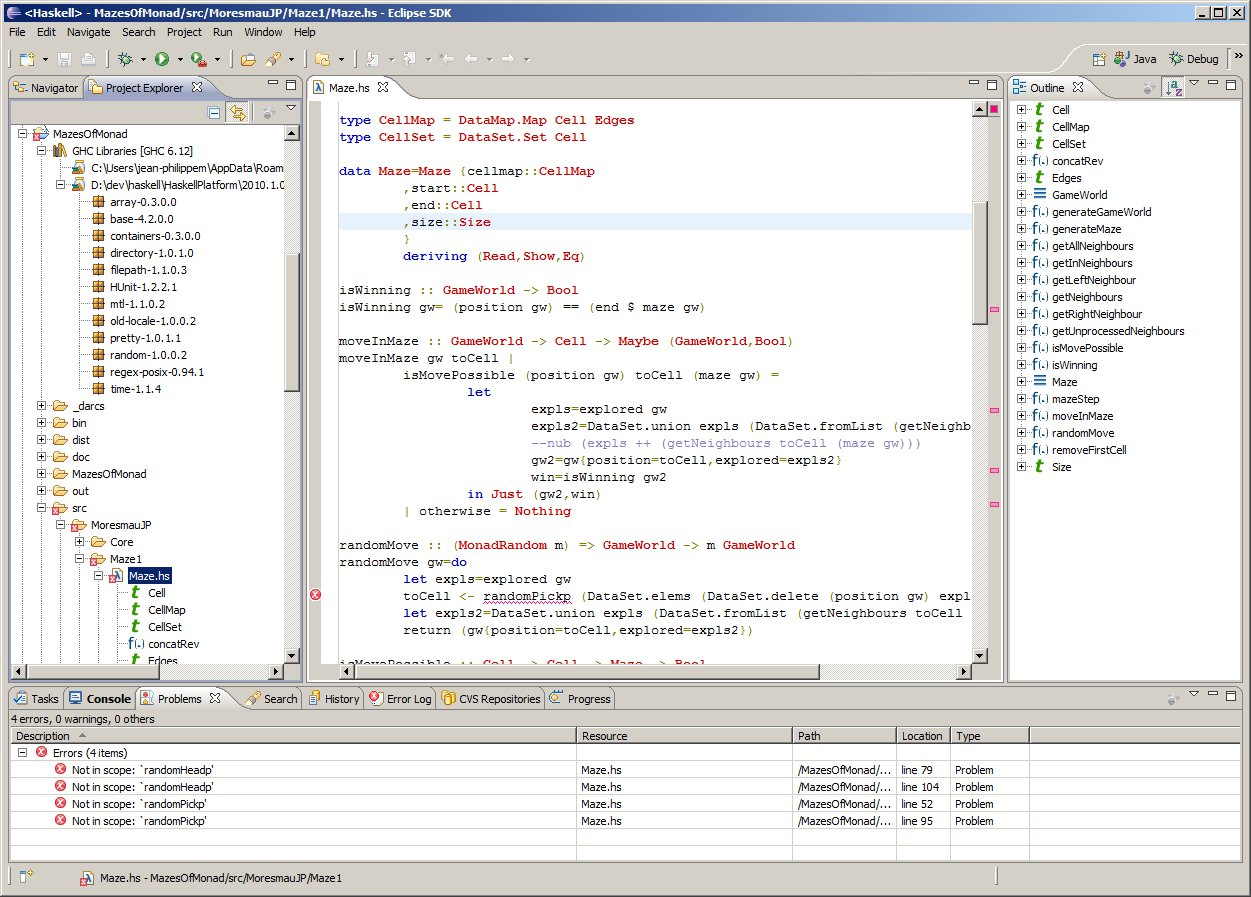
\includegraphics[scale=0.26]{Haskell1.jpg}
	\caption{Some Haskell code in a compiler.}
\end{figure}

This template has been designed for use in modern systems, but can perhaps be adapted to work on older systems, such as Windows 95. Below is a screenshot of a DOSBox console, an MS-DOS emulator designed to work on several platforms. Windows 95 can be installed into DOSBox, but it is not suggested.

\begin{figure}[ht!]
\centering
	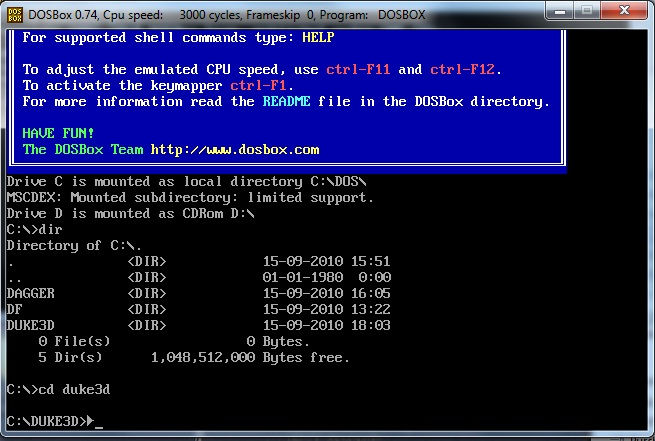
\includegraphics[scale=0.55]{DOSBox1.jpg}
	\caption{The DOSBox console running in Windows 7. The contents of the mounted directory C: are displayed, with the active subdirectory DUKE3D.}
\end{figure}

\section{Specifications in This TAMU \LaTeX ~ Template}

All requirements for theses can be found in the most recent version of the Thesis Manual, available at the OGAPS website. The Thesis Office will be happy to assist you if you have questions about formatting. Questions specific to \LaTeX\ should be directed to \texttt{ogaps-latex@tamu.edu}.

A common question students ask is the placement of a copyright statement at the beginning of a section with reprinted material from a previously printed source. The screenshot below describes how to achieve this. Check the instruction files for more details.

\begin{figure}[ht!]
\centering
	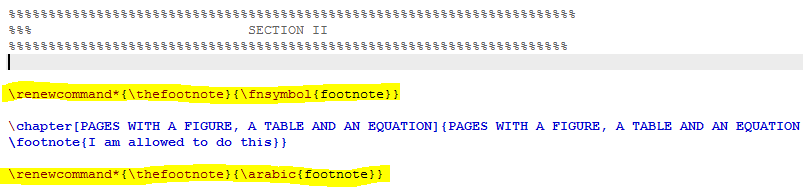
\includegraphics[scale=0.65]{Footnote.png}
	\caption{The inclusion of a copyright statement as a footnote. The lines in yellow help to change to footnote marking scheme.}
\end{figure}

\subsection{Another Test Section}
There should be things here.

%\begin{algorithm}
%Stuff.
%\end{algorithm}

\subsubsection{Test}
Hello, is it me you're looking for?

\subsubsection{Test 2}
There are more things to do.

\subsection{Yet Another One}
She called me late last night to say she loved me so. We insert a slew of figures in the remainder of the document to test the look of the List of Figures.

\begin{figure}[H]
	\centering
	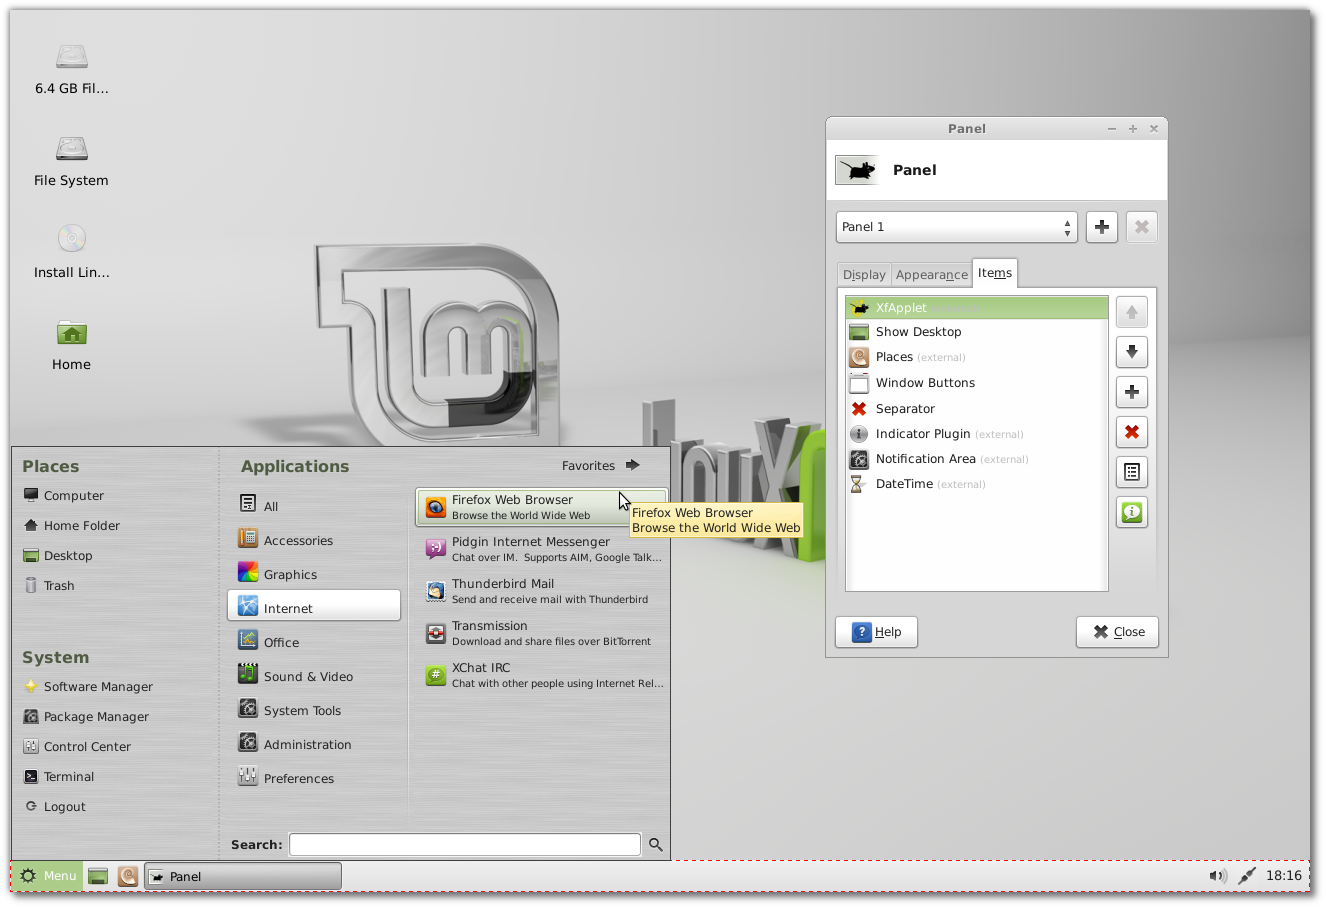
\includegraphics[width=4.25in]{Mint_XFCE.png}
	\caption{Linux Mint 13 with the XFCE desktop environment.}
\end{figure}

Another figure follows below.

\begin{figure}[H]
	\centering
	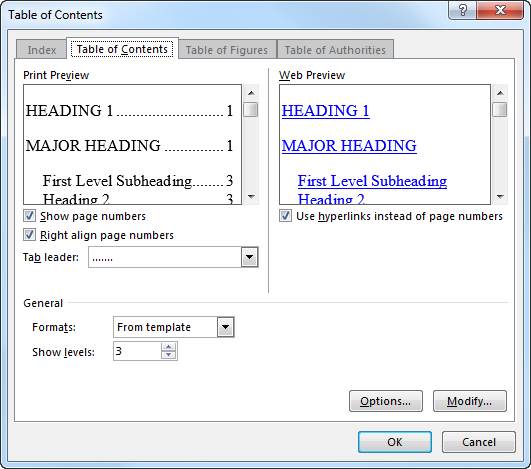
\includegraphics[scale=0.45]{TOC2.png}
	\singlespace
	\caption{The ``Table of Contents" dialog box in Microsoft Word. This must be accessed to properly generate the Table of Contents when using the Recommended Template.}
\end{figure}

Yet another figure follows - the last for this section.

\begin{figure}[H]
	\centering
	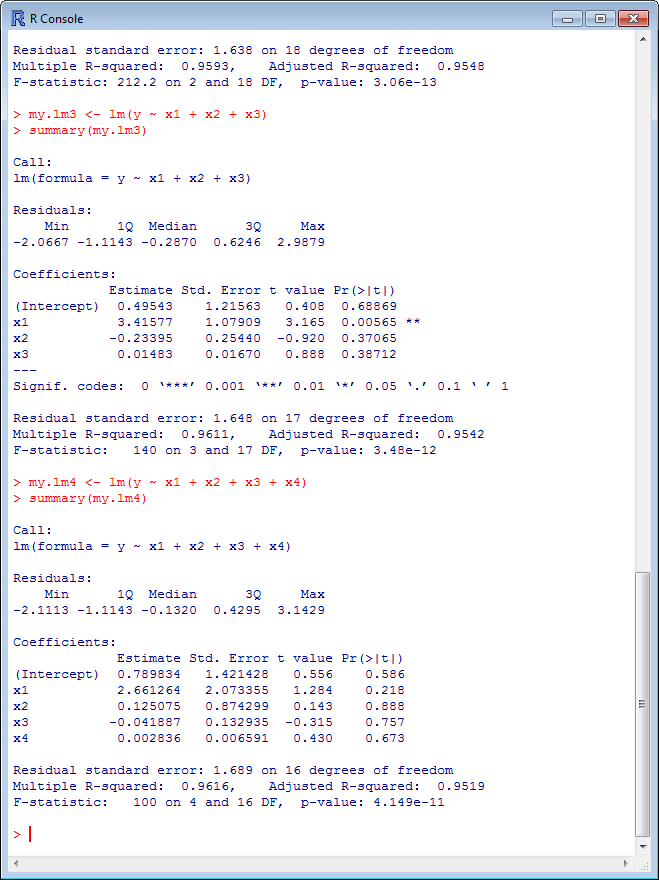
\includegraphics[width=3.75in]{Rachl3.png}
	\singlespace
	\caption{Linear regression on three (top) and four (bottom) independent variables in base R.}
\end{figure}
 
 \subsection{No Surprises Here}
 Insert another song lyric here.

